
%%%%%%%%%%%%%%%%%%%%%%%%%%%%%%%%%%%%%%%%%%%%%%%%%%%%%%%%%%%%%%%%%%%%%%%%
%
% Chapter 3
%

\chapter{DESIGN OF GAME STRATEGIES}
\label{chap:strategy}
The analysis and design of game strategies in this project were a team effort, that incorporated ideas from former works in \cite{FanZhang2013, MingmingCai2013, ChaoLuo2013}. My contribution in this chapter includes developing the cooperative strategy, and improving the competitive strategy.


\section{Cooperative Strategy}
In the cooperative game, we want to maximize the throughput for all the radios in a group. Consequently, our radio should avoid transmitting on parts of the band that other teams are using. Since no prior knowledge of other radios can be used, a spectrum analyzer to sense the usage of the spectrum was chosen based on the topology of the radios as shown in Figure \ref{fig:CooperativeNodeAssignement}. Since most of the signal energy from each radio is on the source side, spectrum sensing on the source side will result in better accuracy.

In most papers discussing spectrum sharing, the synchronization between the source and destination is not considered. However, in a real pair of radios, if the destination does not know which sub-bands are used, it cannot apply an appropriate filter to reduce interference. In our design, a state machine is used to synchronize the source and destination, which has been successfully developed in \cite{FanZhang2013}. The state machine packs the decision into a control packet, and then transmits the control packet to the receiver with 200 kHz-bandwidth and a 64-tone OFDM signal in four different center frequencies across the 5 MHz bandwidth. The limited energy is focused in a very narrow band, and the state machine's signal has very high SIR. Tests show that the state machine is reliable. Technical details on the state machine can be found in \cite{FanZhang2013}.

Feedback can significantly improve the radio performance, and it is also part of our cooperative radio design. Like the state machine, a narrow-band signal is used to increase the SIR. Detailed information on the feedback is discussed in Chapter \ref{chap:strategyAnalysis}.

Figures~\ref{fig:CooperativeStrategy} and \ref{fig:CooperativeCycle} shows the high level algorithm. The four states of the algorithm are spectrum sensing, control packet, feedback, and data transmission. More details on the spectrum sensing is studied in Chapter \ref{chap:spectrumAnalysis}.

\begin{figure}[tpb]
  \begin{center}
    \centerline{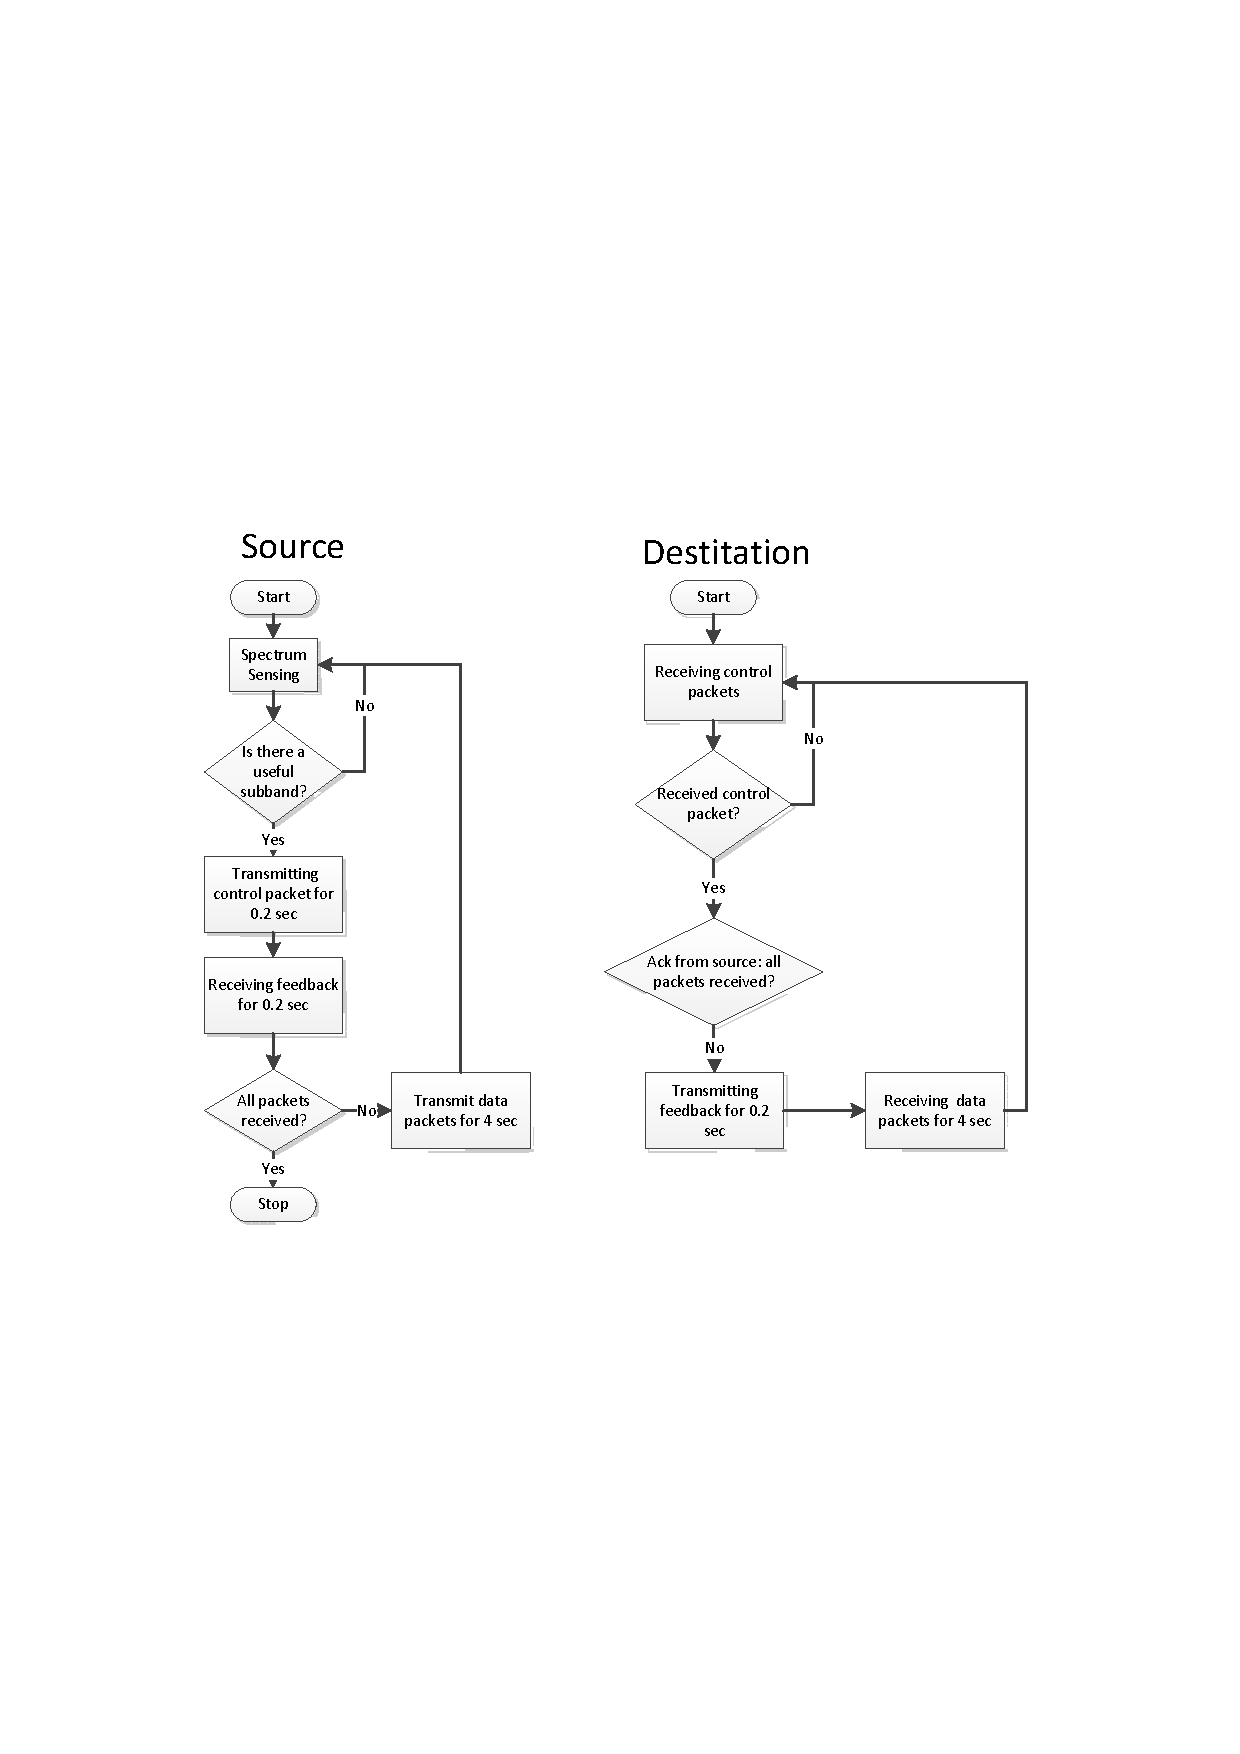
\includegraphics[width=160mm]{CooperativeStrategy.pdf}}
    \caption{Cooperative Strategy}
    \label{fig:CooperativeStrategy}
  \end{center}
\end{figure}

In the control packet state, the source sends 125 control packets, each with same content, through 200 kHz OFDM signal. Each packet has a duration of about 1.8 $ms$. Once the destination receives one of the control packets, it moves to the next state.

In the feedback state, the destination sends feedback packets. From the spectrum sensing results, the center frequency is determined to be the band that has the lowest interference. Both the source and destination choose the largest available band to transmit the feedback packet.

In the data transmission state, 512 tones are divided into 16 sub-bands, each containing 30 tones as discussed in Section \ref{coopPhysicalLayer}. Each sub-band transmits one physical-layer packet. The total data transmission time is about 4 seconds. The total non-data transmission time, including spectrum sensing, synchronization by the state machine, feedback, and switching time, is about 1 second.

In the GNU Radio software, a flow graph consists of the signal processing blocks and the connection among the blocks. Each flow graph needs hundreds of milliseconds to be constructed and also hundreds of milliseconds to be destroyed. Multiple flow graphs can exist in computer's memory at the same time, but only one can run in the CPU at a time. Switching among flow graphs can be achieved by locking the current running flow graph and then unlocking the flow graph to be run. Locking and unlocking the flow graphs requires a few milliseconds. The transmitter of the USRP can only accept one stream of data as input. Therefore, two blocks that output data to the same transmitter of the USRP cannot be implemented in the same flow graph. In our design of cooperative radio, multiple states need more than one flow graph. Ideally, each state should be implemented in one flow graph to modularize the program. As a result, a smaller number of flow graphs is preferred. Finally, two flow graphs are used for both the source and destination. Figure~\ref{fig:CooperativeCycle} illustrates the process of one cooperative cycle, where the dotted box represents one flow graph. In order to reduce the switching time, switching between the flow graphs is conducted by locking and unlocking operation rather than by the construction and destruction of flow graphs.

\begin{figure}[tpb]
  \begin{center}
    \centerline{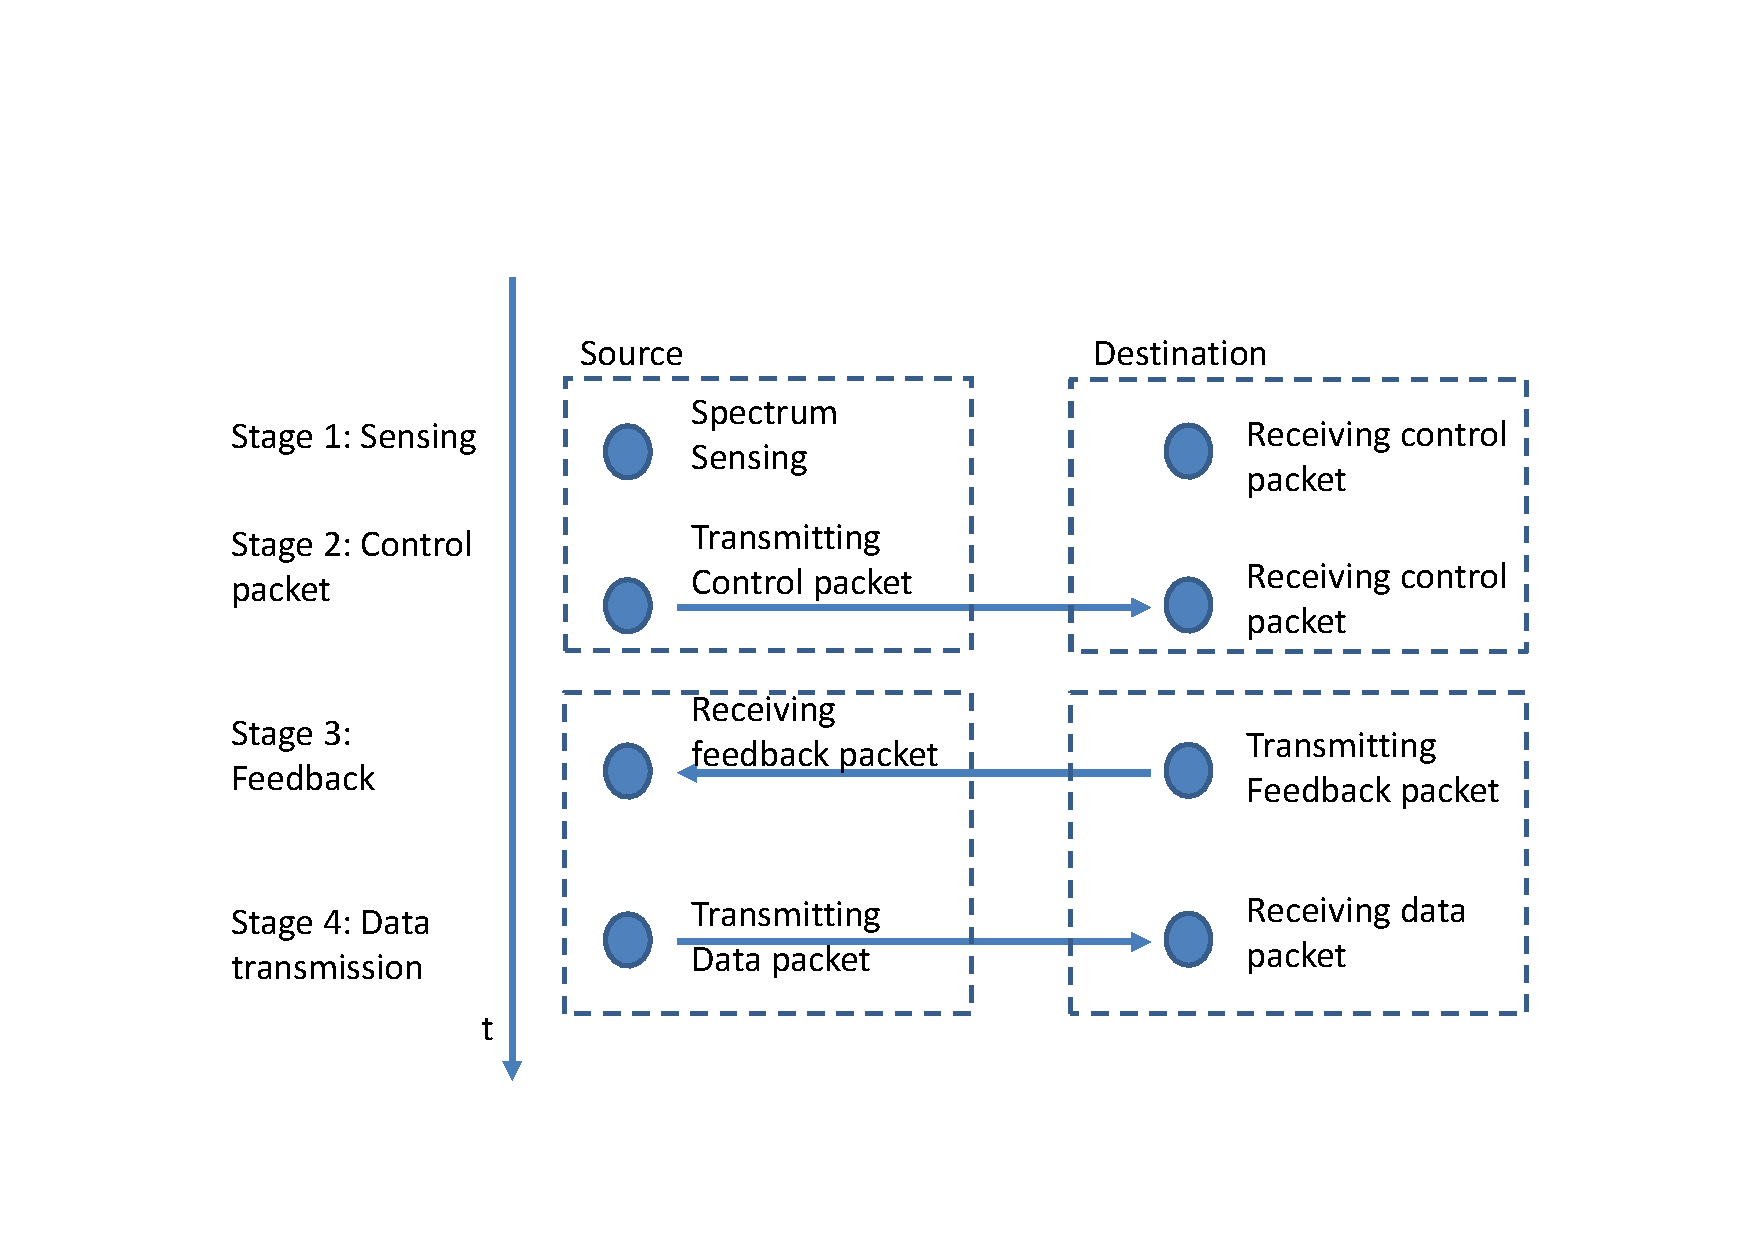
\includegraphics[width=160mm]{CooperativeCycle.pdf}}
    \caption{One Cooperative Cycle. The dotted boxes represent one flow graph.}
    \label{fig:CooperativeCycle}
  \end{center}
\end{figure}


\section{Competitive Strategy}
\label{comptititveStrategy}
In Figure~\ref{fig:CompetitiveNodeGeometryFinalRound}, S1 is farther away from the competitor nodes S2 and D2 than D1, so the reverse link is subject to less interference than the forward link. As a result, the reverse link is more reliable. Therefore, feedback can be applied to increase the reliability and efficiency of the forward link in the competitive match. Generally, the two ways to implement the feedback are time division duplex (TDD) and frequency division duplex (FDD).

In FDD systems, the forward and the reverse links occupy different frequency bands. In TDD systems, the forward and the reverse links share the spectrum with time multiplexing. FDD systems need a large guard band to ensure no interference between the forward link and the reverse link. However, we must take into account the close proximity of the transmitter and receiver antennas. A front-end filter would be needed to implement FDD, but no such front-end filter exists in USRP. If FDD is implemented with the USRP, the front-end amplifier will be saturated by the signal from the transmitter at the same USRP.

Consequently, TDD will be used to implement the feedback. The TDD sync can be controlled by either the source or destination. Since the reverse link is more reliable than the forward link, we let the destination node control the TDD sync by periodically sending the TDD preamble containing TDD sync information to the source. More details on TDD will be discussed in Chapter \ref{chap:TDD}.

We define a TDD frame as the transmission period of a TDD cycle. A TDD sub-frame is defined as a collection of data that is synchronized by one preamble in OFDM. In a TDD frame, 100 sub-frames will be sent through the forward link and 10 sub-frames will be sent through the reverse link. So our system keeps a 10:1 time ratio between the forward and reverse link. The time of each frame is 206 $ms$.

In both the forward link and reverse link, 512 subcarriers are divided into 8 sub-bands, each containing 60 subcarriers (the unused subcarriers are reserved for the DC tone and side lobes). We refer to the data transmitted in a sub-band of a sub-frame as a physical-layer packet, and its size is 256 bytes if QPSK is used. A 32-bit CRC check is attached to each physical-layer packet.

Channel coding is used in the forward link. Specifically, repetition codes with code rate 1/2 and 1/4 are allowed. A MAC payload is defined as the data before it is encoded into a physical-layer packet. In other words, an encoded MAC payload is a physical-layer packet. A 1440-byte packet from the server is divided into smaller pieces called sub-packets to fit the size of a MAC payload. A header is used to distinguish different sub-packets. As a result, a MAC payload consists of a header and its corresponding sub-packet. When different coding schemes are used, the size of the MAC payloads will vary, but the structure of the header will not. More details about the packet management will be introduced in Chapter \ref{chap:spectrumAnalysis}

Four bit rates are used based on the channel coding and modulation, which include uncoded QPSK (rate 1), QPSK with rate 1/2 repetition code, BPSK with 1/2 repetition code, and BPSK with 1/4 repetition code. Each sub-band can choose individually which bit rate is used based on the channel quality. On the destination side, a length 100 moving packet success rate is calculated in real time for each sub-band. If the packet success rate for a sub-band is larger than 90 percent, the destination will order the source via a control signal to switch the sub-band to a higher bit rate until the highest rate, uncoded QPSK is achieved. If the packet success rate is less than 50 percent, the destination will order the source to switch the sub-band to a lower bit rate until the lowest rate, BPSK with 1/4 repetition code, is achieved. If the packet success rate is 0 at BPSK with 1/4 repetition code, the destination will order the source to shut down that the sub-band to save power for other sub-bands. However, to make sure no large spectrum is left without interference to our competitor, consecutive sub-bands will not be shut down simultaneously. Index the sub-band as sub-band $1,2,...,8$. The algorithm states that if sub-band $i-1$ is shut down, sub-band $i$ is not shut down, for $i=2,3,...8$.



